\section{Simulation of Path Planner}

The same autopilot that was used for simulating the controller will be used when simulating the path planner. A path follower will be used to give course commands to the autopilot during simulation, while the rest of the states will be controlled only by the autopilot.


\subsection{Path Follower}
\label{ch:path_follower}

Two different path followers will be used in this simulation. The first path follower will be used to follow the Dubins path, while the second will be used to follow the continuous path that is generated as an improvement to the Dubins path.

The strategy used to follow Dubins path will be based on two algorithms presented in \cite{suaBEARD} by Beard \& McLain. The two algorithms are used to follow straight and curved line paths.

In order to follow straight line paths, the algorithm uses the position and heading of the aircraft, the previous waypoint and the direction from the previous to the next waypoint as input. The previous waypoint and direction to the next waypoint are given as output from the algorithm generating Dubins path described in chapter \ref{ch:dubins_path}. The new course is calculated so that the aircrafts position will converge towards the original path.

The algorithm for following circular paths is based on following perfect circles. Therefore it takes center and radius of the circle, the direction to orbit the circle, and the current position and heading of the aircraft. The heading calculated here will also ensure that the aircrafts position converges to the cirular path.

The altered path is based on the route that is flown in the first simulation, and will therefore not consist of circular arcs and straight lines. Instead the path will be a continuous path which requires a different path follower. The path follower will be based on the principles of Line Of Sight (LOS) steering laws presented by Fossen \cite{fartoyFOSSEN}.

Enclosure-based steering is LOS principle that considers a circle with radius $R$ enclosing the vehicle, which represents the LOS distance. Assuming that the radius is suffieciently large compared to the vehicle's distance from the path, the circle will intersect the path at two different points. One of the points will be in the direction of the vehicle, denoted $x_{los}$ and $y_{los}$. This is the point the vehicle will be directed to, and the course to that point can be expressed as \cite{fartoyFOSSEN}:

\begin{equation}
	\chi_d(t) = \text{atan2}(y_{los} - y(t), x_{los} - x(t))
\end{equation}

where $x(t)$ and $y(t)$ is the vehicle's current position. Using Pythagoras theorem, the points $x_{los}$ and $y_{los}$ can be found as:

\begin{equation}
	[x_{los} - x(t)]^2 + [y_{los} - y(t)]^2 = R^2
\end{equation}

where $R$ is the chosen LOS distance.


\subsection{Simulation Setup}

The simulation was performed using the same Simulink and Matlab setup as previously, using the path followers to generate the desired course angle. The Dubin's path that will be used as a reference is shown in figure \ref{fig:dubins_reference}.

\begin{figure}[!ht]
    \centering
    \makebox[\textwidth][c]{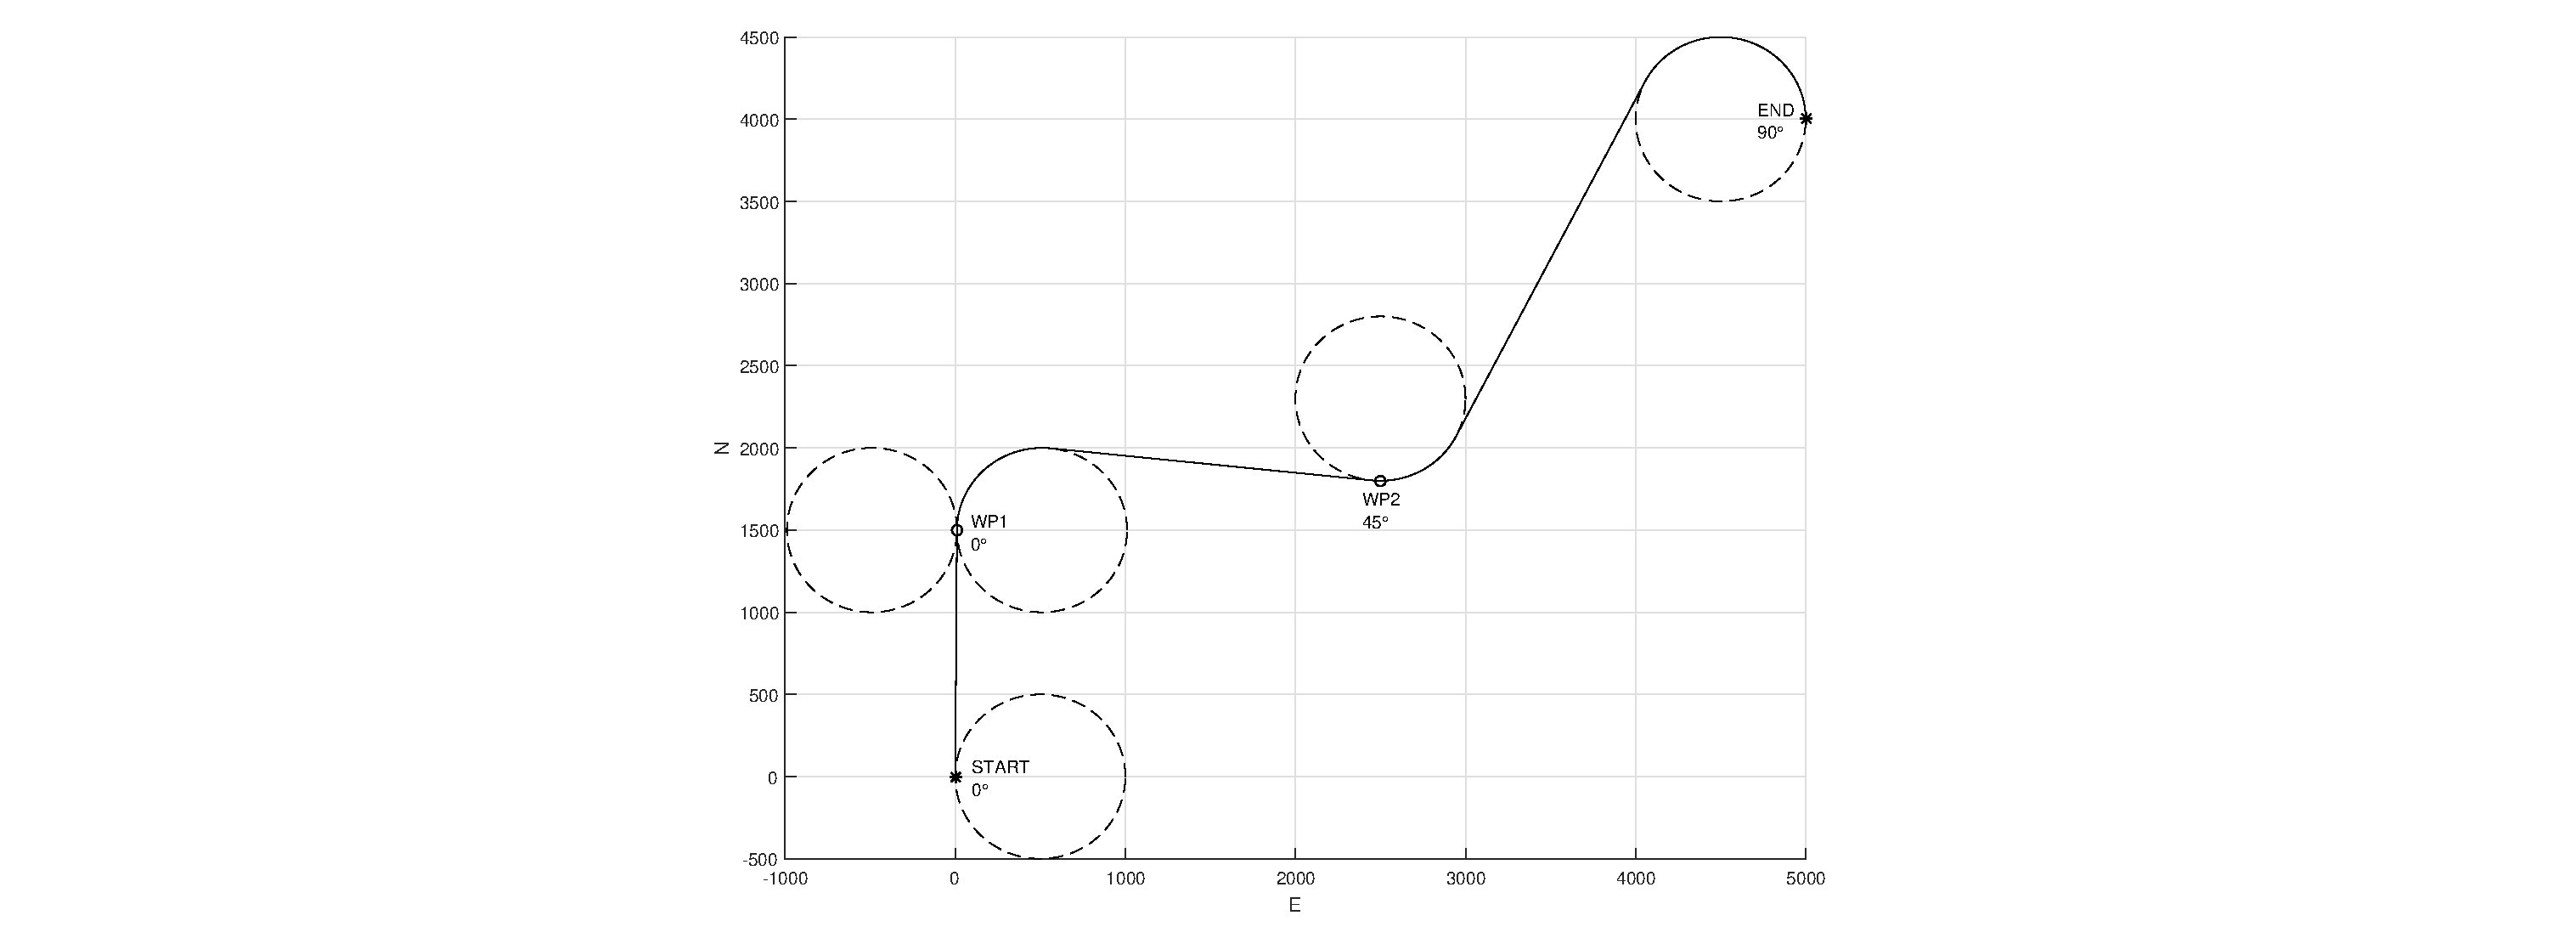
\includegraphics[width=2.2\textwidth, keepaspectratio=true]{dubins_reference.eps}}
    \caption{The path that will be simulated, with the direction associated with every waypoint.}
	\label{fig:dubins_reference}
\end{figure}

The radius of the circles in the Dubins path was chosen to $600$ m, and is the same for every waypoint. IF it is assumed that there is no wing and no sideslip, the equation for a coordinated turn becomes \cite{suaBEARD}:

\begin{equation}
	R = \frac{V_g^2}{g\text{tan}(\phi)}.
\end{equation}

With $R$ set to $600$ m, and the airspeed equal to the groundspeed at $35$ m/s, the corresponding roll $\phi$ is about $15\degree$. This seems reasonable, as it is not expected that a UAV performing ground observation will be performing high dynamic maneouvres. The LOS distance was set to $200$ m by trial and failure.


\subsection{Result: Path Following}

Figure \ref{fig:first_run_path} and figure \ref{fig:first_run_turns} shows the result of the simulation when the UAV follows the generated Dubins path that is to be observed. The aircraft follows the observation path closely, and in turns it drifts slightly off and takes the outer turn. 

\begin{figure}[!ht]
    \centering
    \makebox[\textwidth][c]{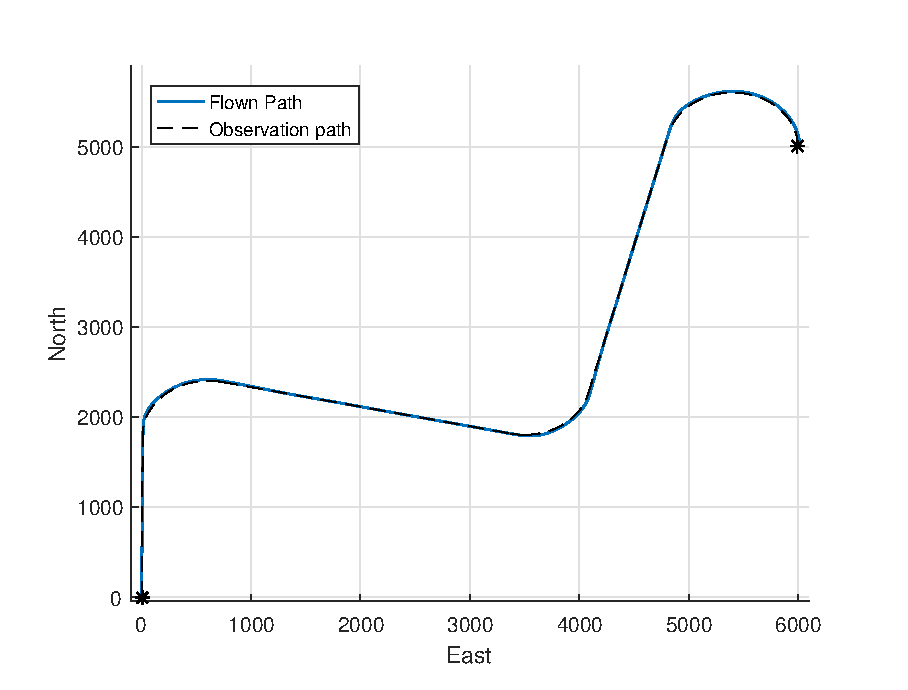
\includegraphics[width=1.2\textwidth, keepaspectratio=true]{../../results/path/first_run_path.eps}}
    \caption{The path flown by the aircraft on the first run.}
	\label{fig:first_run_path}
\end{figure}

\begin{figure}[!ht]
    \centering
    \makebox[\textwidth][c]{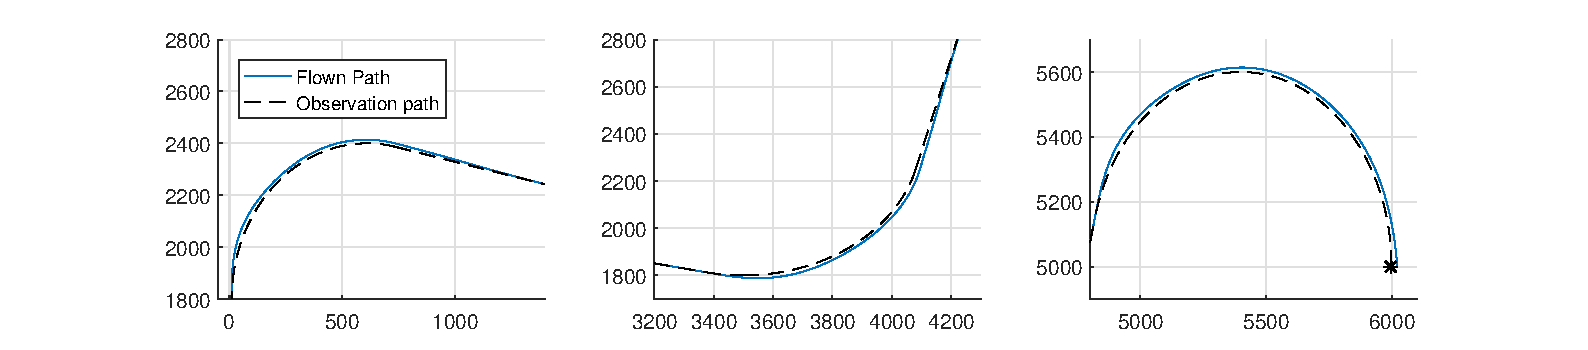
\includegraphics[width=1.8\textwidth, keepaspectratio=true]{../../results/path/first_run_turns.eps}}
    \caption{The path the aircraft took through the turns on the first run.}
	\label{fig:first_run_turns}
\end{figure}

\begin{figure}[!ht]
    \centering
    \makebox[\textwidth][c]{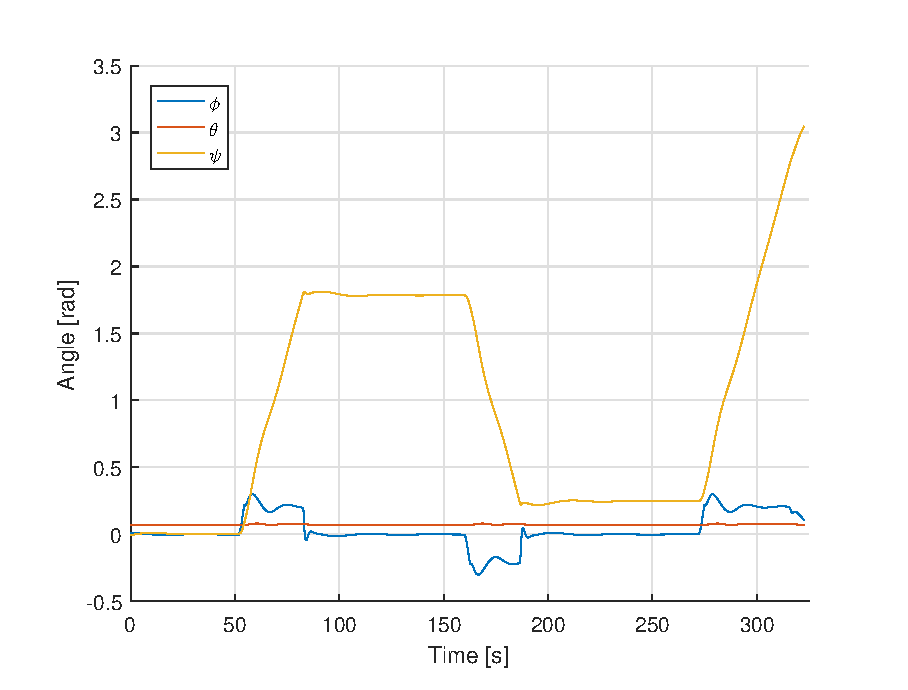
\includegraphics[width=1.2\textwidth, keepaspectratio=true]{../../results/path/first_run_states.eps}}
    \caption{The attitude states of the aircraft during the first run.}
	\label{fig:first_run_states}
\end{figure}

Figure \ref{fig:first_run_states} shows the attitude states of the aircraft during the flight, and shows that the roll $\phi$ is just below $0.25$ rad for each turn, which is about $15 \degree$ as predicted previously. However, it can be seen that $\phi$ varies during the course changes, meaning that the aircraft is not doing a perfectly smooth turn. When using equation (\ref{eq:roll_impact}) to calculate how the path should be altered, these uneven turns will cause the path to be uneven as well. The altered path is shown together with the original flown path in figure \ref{fig:altered_vs_flown}. The figure shows some "NUDGES" due to the uneven turn, mainly at the beginning and end of the turns.

\begin{figure}[!ht]
    \centering
    \makebox[\textwidth][c]{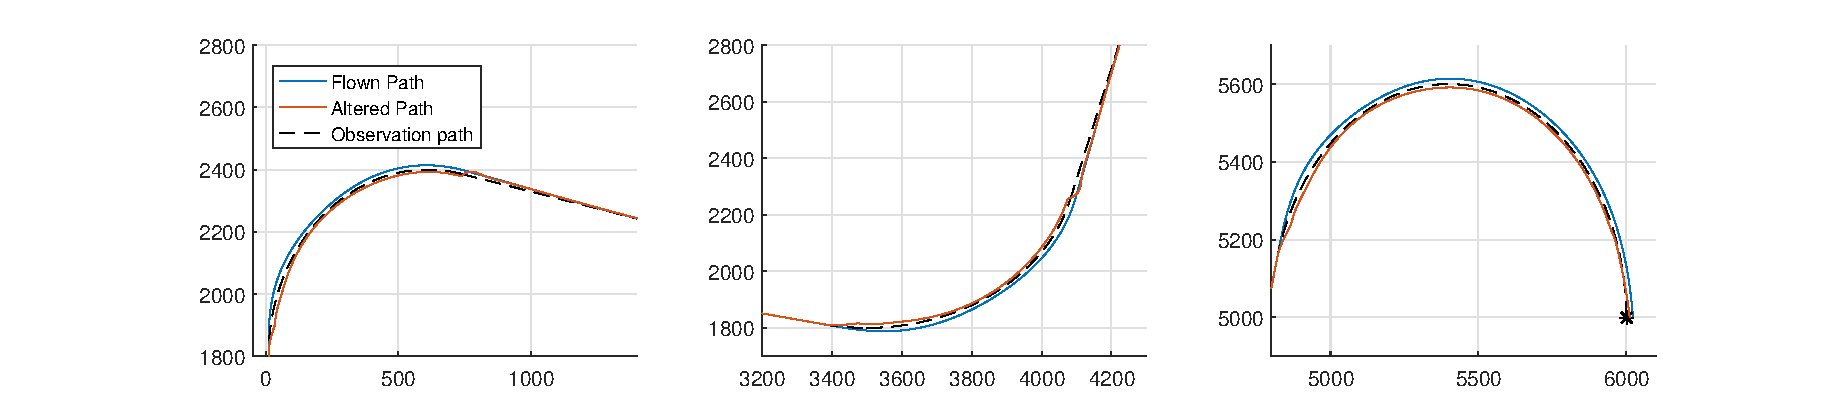
\includegraphics[width=1.8\textwidth, keepaspectratio=true]{../../results/path/altered_vs_flown.eps}}
    \caption{The figure shows how the altered path is compared to the flown path. Only the turns are shown as they are matching during the straight levelled sections.}
	\label{fig:altered_vs_flown}
\end{figure}

The altered path is supposed to counteract the slow and more constant changes in roll during a turn. The changes in roll caused by the uneven turn are much faster than than the slow changes. This means that the unwanted changes in roll can be removed by passing the signal through a low-pass filter. The result of altering the path with the low-pass filtered $\phi$ is shown in figure \ref{fig:filtered_vs_unfiltered}, and the result that the new path is smoother than the first one.

\begin{figure}[!ht]
    \centering
    \makebox[\textwidth][c]{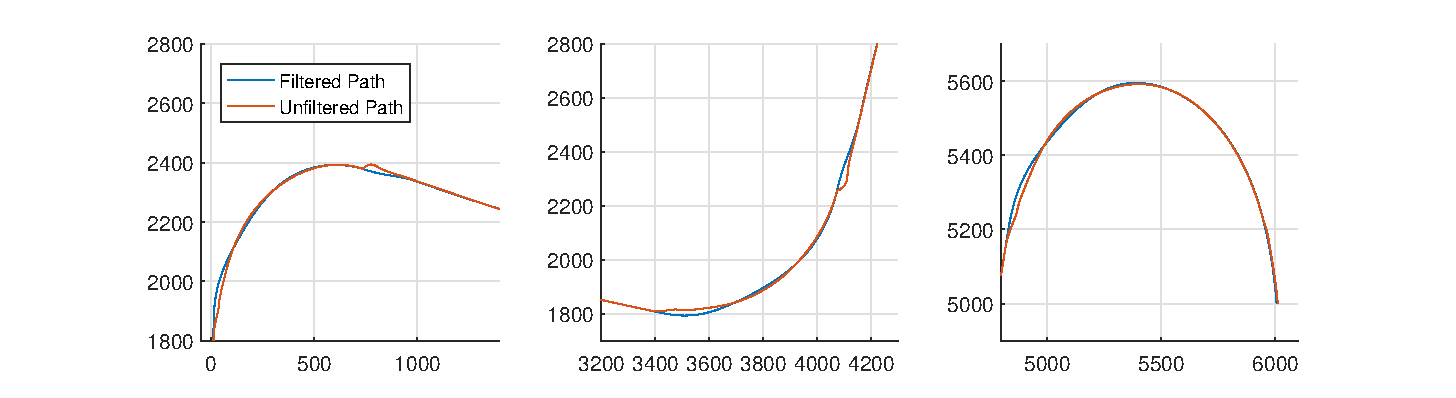
\includegraphics[width=1.8\textwidth, keepaspectratio=true]{../../results/path/filtered_vs_unfiltered.eps}}
    \caption{The path created by using the filtered signal for $\phi$ compared to using the unfiltered.}
	\label{fig:filtered_vs_unfiltered}
\end{figure}

The result of the simulation when following the altered path is shown in figures (\ref{fig:second_run_path}), (\ref{fig:second_run_turns}) and (\ref{fig:second_run_states}). It can be seen that instead of taking the outer path during turns, the aircraft now takes the inner turn which is what we want. It can be seen that $\phi$ is still uneven during turns, and about the same value as during the first run.

\begin{figure}[!ht]
    \centering
    \makebox[\textwidth][c]{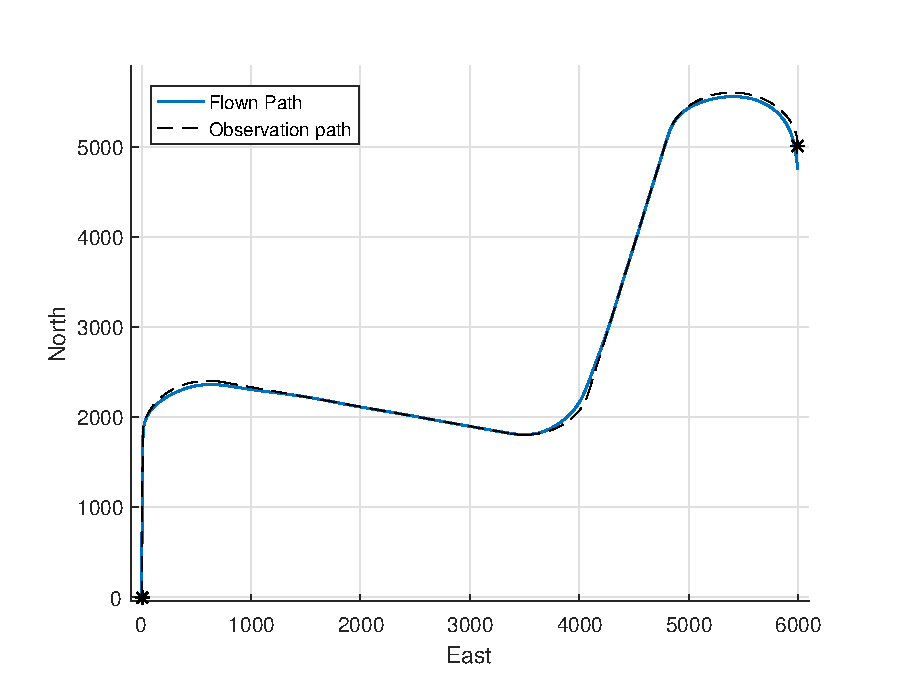
\includegraphics[width=1.2\textwidth, keepaspectratio=true]{../../results/path/second_run_path.eps}}
    \caption{The path flown by the aircraft when following the altered path.}
	\label{fig:second_run_path}
\end{figure}

\begin{figure}[!ht]
    \centering
    \makebox[\textwidth][c]{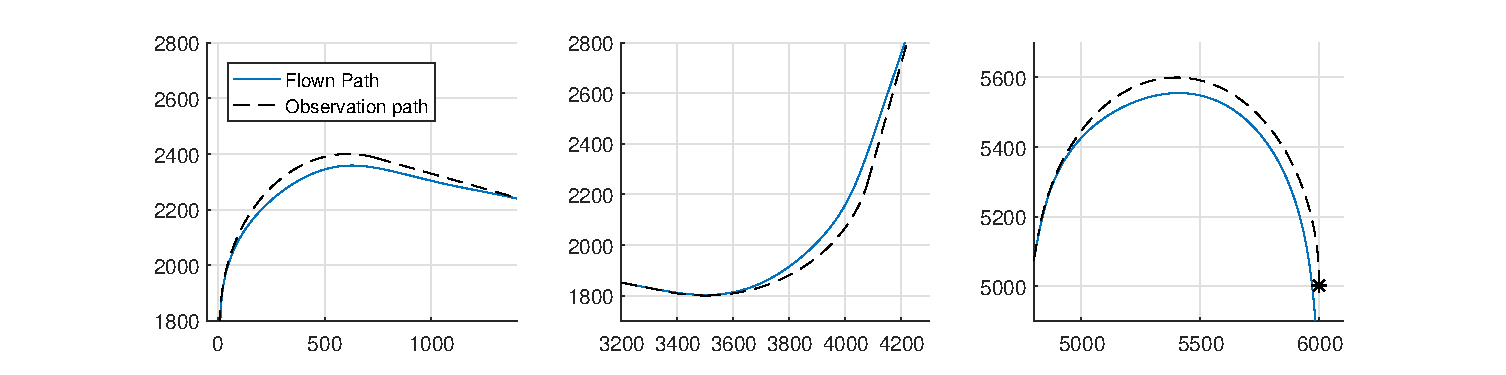
\includegraphics[width=1.8\textwidth, keepaspectratio=true]{../../results/path/second_run_turns.eps}}
    \caption{The path the aircraft took through the turns when following the altered path.}
	\label{fig:second_run_turns}
\end{figure}

\begin{figure}[!ht]
    \centering
    \makebox[\textwidth][c]{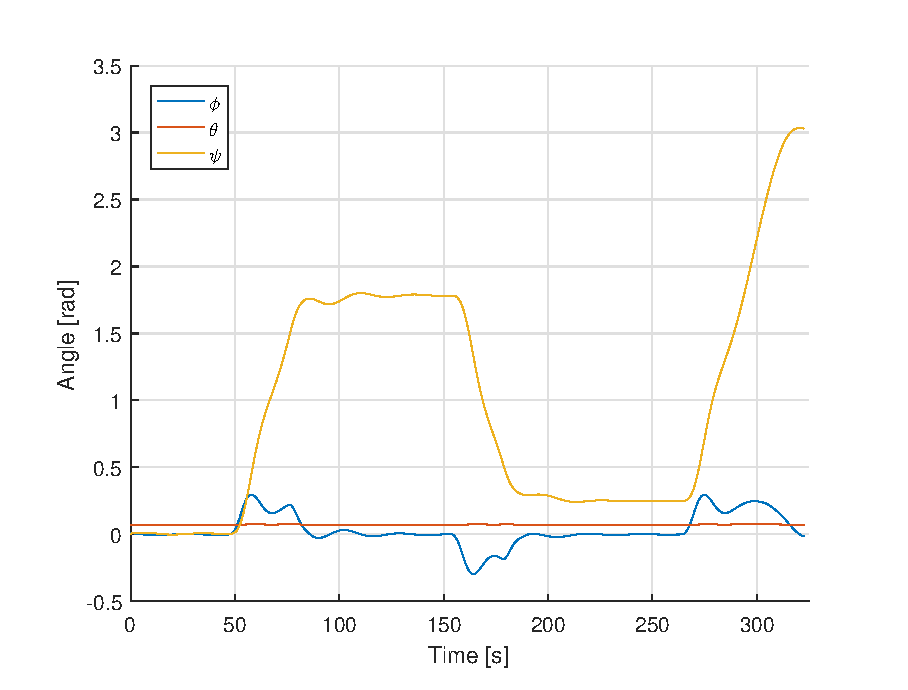
\includegraphics[width=1.2\textwidth, keepaspectratio=true]{../../results/path/second_run_states.eps}}
    \caption{The attitude states of the aircraft when following the altered path.}
	\label{fig:second_run_states}
\end{figure}


\subsection{Result: Camera Footprint}

The camera footprint for the original path is shown in figures \ref{fig:first_camera_path} and \ref{fig:first_camera_turns}. While the camera footprint is positioned fairly straight above the observation path, the observation path is outside of the camera footprint during turns. The footprint drifts completely off the observation path in the beginning of the turn, but it catches up after the initial "NUDGE". This matches the results from the previous section where the roll $\phi$ was the highest in the beginning of the turn. There is also a big change in $\phi$ at the end of the turn, which leads to a large movement of the camera footprint.

\begin{figure}[!ht]
    \centering
    \makebox[\textwidth][c]{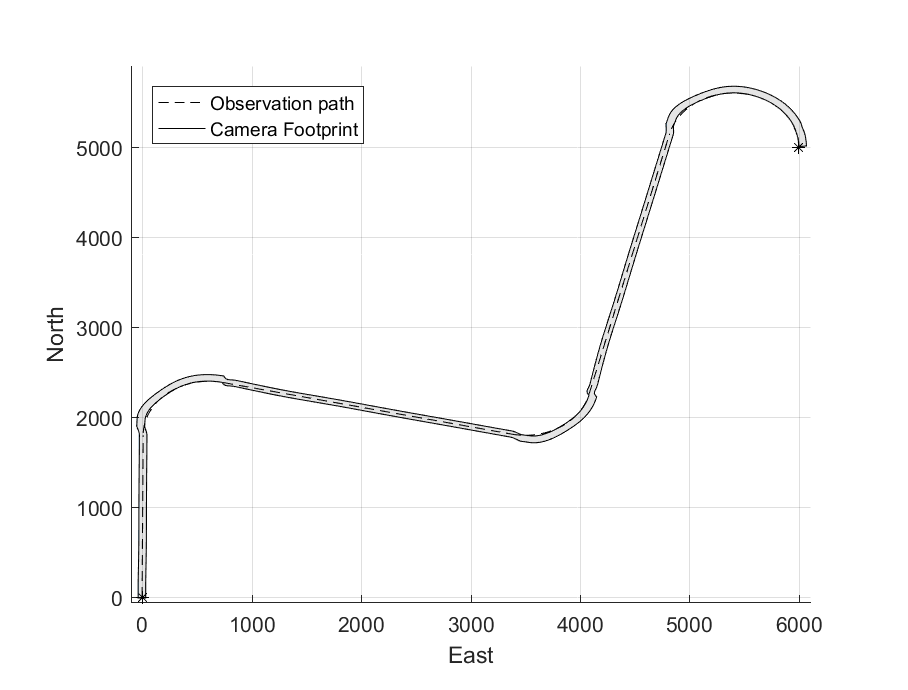
\includegraphics[width=1.2\textwidth, keepaspectratio=true]{../../results/path/first_camera_path.eps}}
    \caption{The camera footprint during simulation of the first path.}
	\label{fig:first_camera_path}
\end{figure}

\begin{figure}[!ht]
    \centering
    \makebox[\textwidth][c]{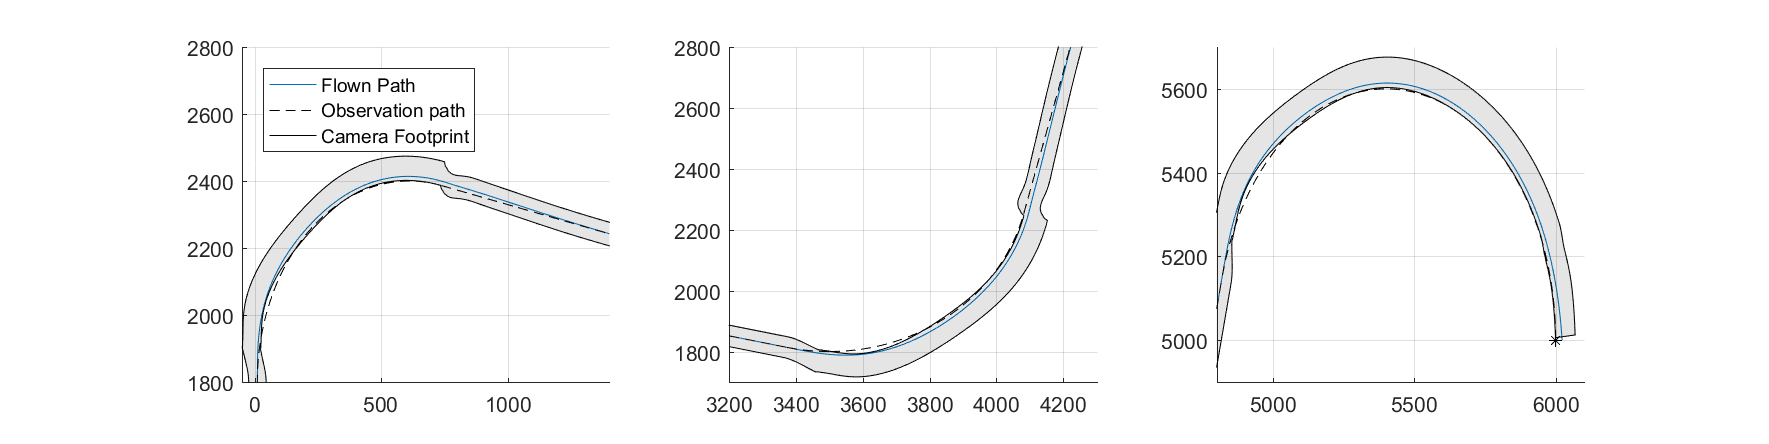
\includegraphics[width=1.8\textwidth, keepaspectratio=true]{../../results/path/first_camera_turns.eps}}
    \caption{The camera footprint in turns during the simulation of the first path.}
	\label{fig:first_camera_turns}
\end{figure}

\begin{figure}[!ht]
    \centering
    \makebox[\textwidth][c]{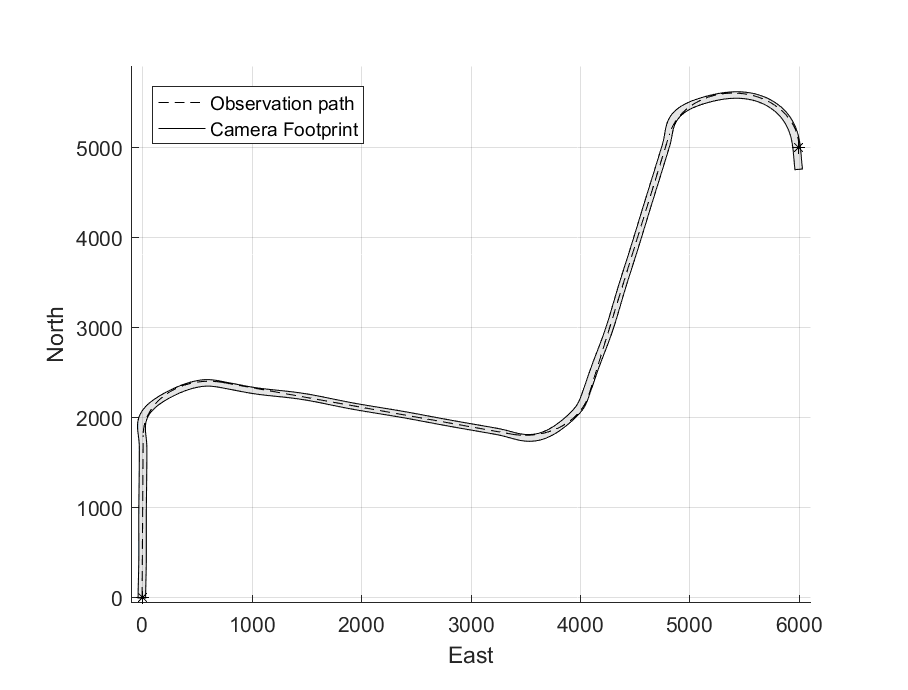
\includegraphics[width=1.2\textwidth, keepaspectratio=true]{../../results/path/second_camera_path.eps}}
    \caption{The camera footprint during simulation of the altered path.}
	\label{fig:second_camera_path}
\end{figure}

\begin{figure}[!ht]
    \centering
    \makebox[\textwidth][c]{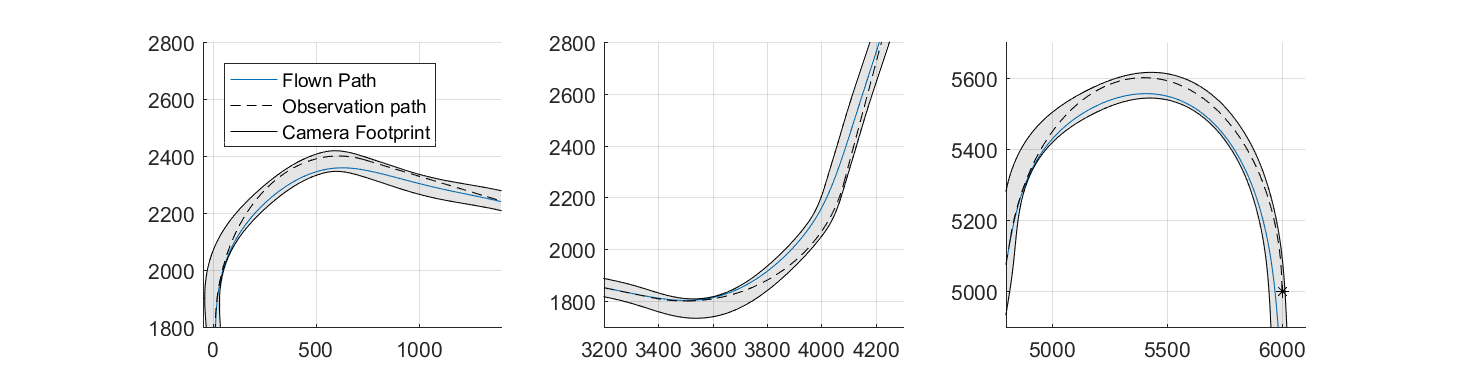
\includegraphics[width=1.8\textwidth, keepaspectratio=true]{../../results/path/second_camera_turns.eps}}
    \caption{The camera footprint in turns during the simulation of the altered path.}
	\label{fig:second_camera_turns}
\end{figure}

\begin{figure}[!ht]
    \centering
    \makebox[\textwidth][c]{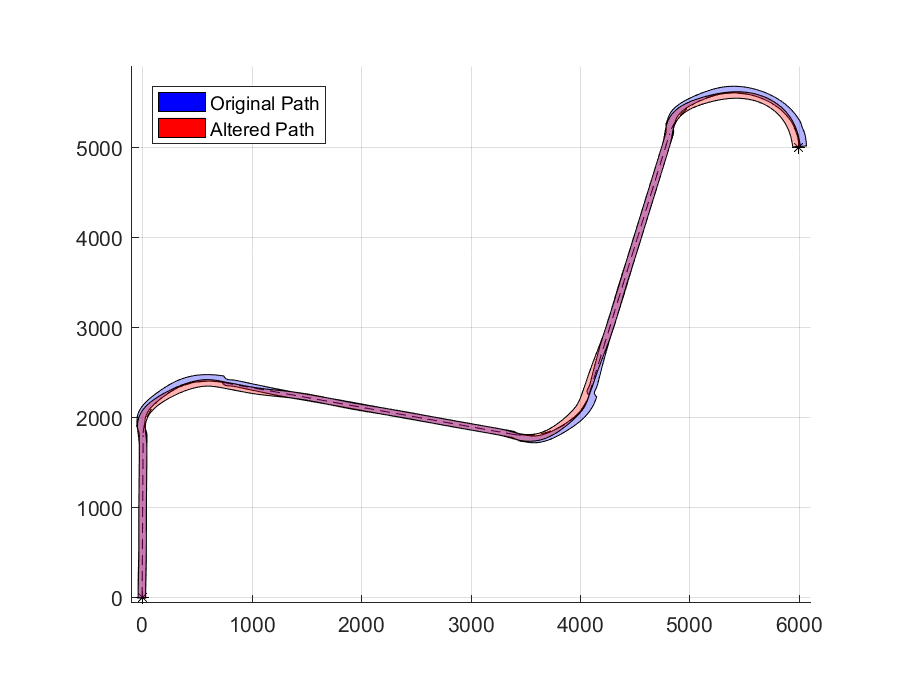
\includegraphics[width=1.2\textwidth, keepaspectratio=true]{../../results/path/both_camera_path.eps}}
    \caption{The camera footprint during simulation of the altered path.}
	\label{fig:both_camera_path}
\end{figure}

\begin{figure}[!ht]
    \centering
    \makebox[\textwidth][c]{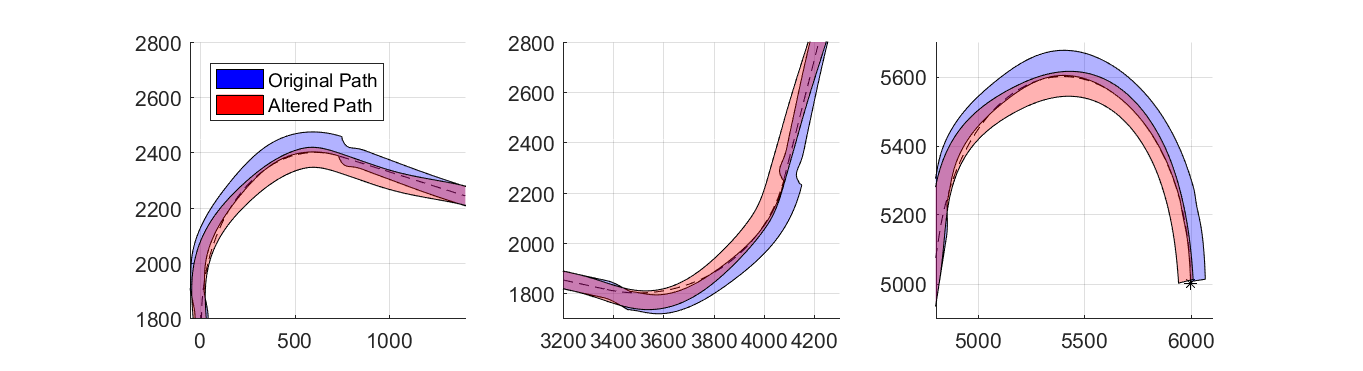
\includegraphics[width=1.8\textwidth, keepaspectratio=true]{../../results/path/both_camera_turn.eps}}
    \caption{The camera footprint in turns during the simulation of the altered path.}
	\label{fig:both_camera_turns}
\end{figure}